Inizialmente, il dataset delle traiettorie è composto da un insieme di punti aventi le seguenti caratteristiche:
una dimensione temporale espressa in secondi, due coordinate spaziali per determinare la sua posizione rispetto a un sistema di coordinate polari e
infine un identificatore di traiettoria. A queste dimensioni possono essere poi aggiunte altre informazioni, che possono essere potenzialmente considerate durante questo primo passaggio dell'algoritmo.

Scopo di questa prima fase dell'algoritmo \textit{Cu.Te} è determinare un sistema di riferimento per i punti all'interno del dataset ed esprimere questi ultimi in
relazione al nuovo sistema.

Come indicato nella~\cref{subsec:cute:parameters}, è possibile determinare un sistema di riferimento che più aderisce alle esigenze del problema.
In questo caso la necessità principale in vista della fase di \textit{Colossal Trajectory Mining} è la ridotta dimensionalità dello spazio-tempo rispetto al numero di traiettorie
processate: si rende infatti necessario avere un numero di riferimenti spazio-temporali strettamente inferiorie alle traiettorie presenti nel database.

L'idea per risolvere questa esigenza è la divisione della superficie spazio-temporale in celle omogenee per range. Dato l'intero volume dello spazio-tempo
coperto dalle traiettorie nel dataset, questo viene partizionato in parallelepipedi di medesime dimensioni. Una cella \textit{c} è un parallepipedo, generato dal
partizionamento dello spazio-tempo coperto dalle traiettorie, avente un indice univoco.
Questa suddivisione costituisce quindi il nuovo sistema di riferimento del problema, si rende necessario quindi esprimere i punti all'interno del dataset nelle nuove
metriche di questo nuovo sistema.

Partendo dallo spazio, ogni punto di traiettoria, per definizione, determina la propria posizione sulla superficie terrestre utilizzando due coordinate, latitudine e longituidne.
Prendendo in considerazione l'area di un insieme di traiettorie, il processo per la generazione di celle spaziali è il seguente: per prima cosa si determina, mediante
il parametro \textit{s} la dimensione dei lati spaziali di una cella; successivamente si determina una funzione \textit{pointToCell}, tale funzione ha il compito
di restituire, dato un punto, la cella di appartenenza. La cella in questione viene calcolata supponendo di scomporre la superficie terrestre in celle aventi raggio \textit{s}
a partire da Null Island (punto avente latitudine e longituidne pari a zero)~\footnote{\url{https://blogs.loc.gov/maps/2016/04/the-geographical-oddity-of-null-island/}}.
In~\cref{fig:chap-3:milan-cell-division} è possibile vedere un esempio di divisione in celle applicato sulla città di Milano.

\begin{figure}
  \centering
  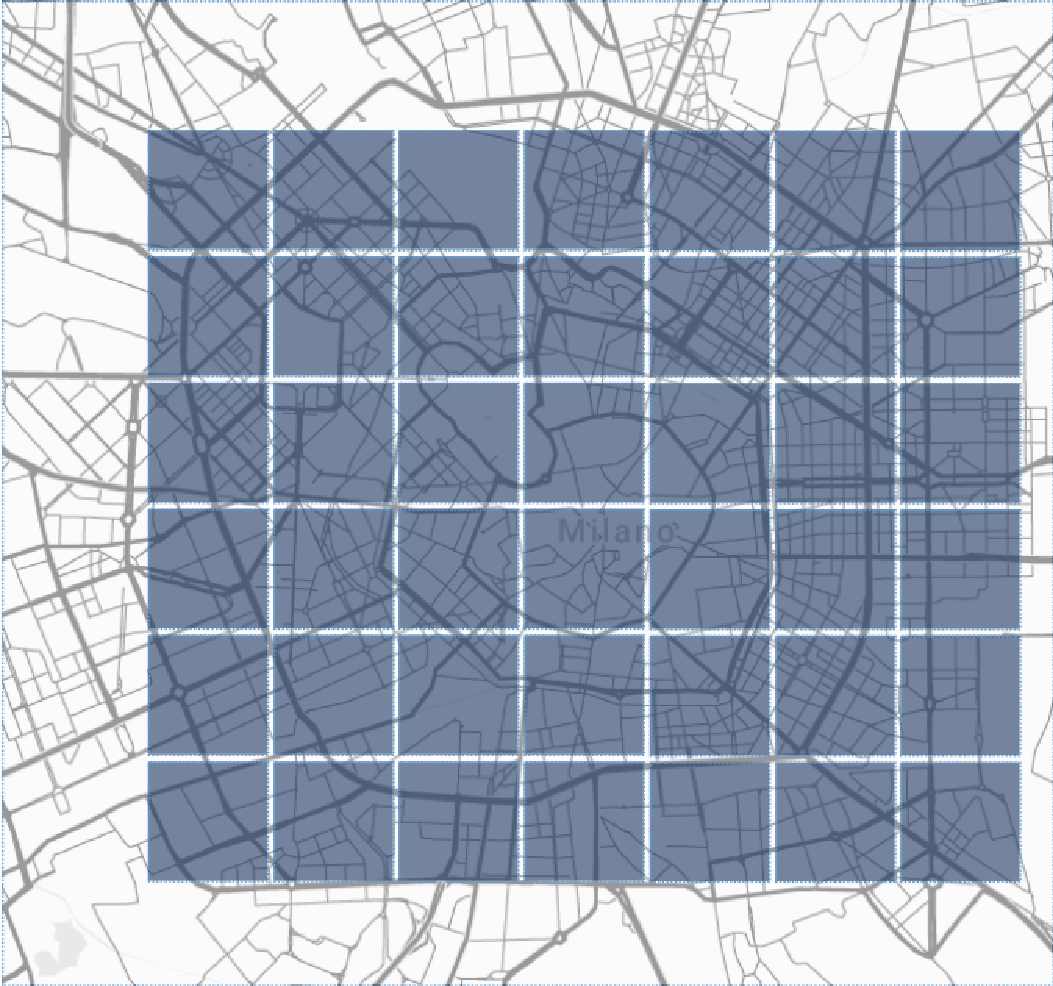
\includegraphics[scale=.6]{/sec-3/MilanCells.pdf}
  \caption{Suddivisione della città di Milano in celle,Fonte:~\url{https://which.souce?}}%
  \label{fig:chap-3:milan-cell-division}
\end{figure}

Per quanto riguarda la dimensione temporale invece, le possibilità a disposizione sono diverse, ma tra tutte si è scelto di supportare due principali scale: una basata sulle ore del giorno mentre l'altra sui giorni della settimana.
Rispetto a una metrica di tempo monotona basata su data e ora di ogni singolo punto, come ad esempio in \textit{G.C.M.P}, una scala circolare ha due vantaggi: il primo riguarda
il supporto a pattern ciclici che verrebbbero ignorati da una metrica monotona e in secondo luogo il ridotto range di valori della scala (da 0 a 23 in caso di scala giornaliera, da 0 a 6 in quella settimanale)
previene l'esplosione nel numero di celle al crescere del dataset.



